\documentclass[12pt]{report}

\usepackage[a4paper,width=150mm,top=25mm,bottom=25mm,bindingoffset=6mm]{geometry}
\usepackage[onehalfspacing]{setspace}
\usepackage{ucs}
\usepackage[table,xcdraw]{xcolor}
\definecolor{mColor1}{rgb}{0.9,0.9,0.9}

\usepackage{fancyhdr}
\pagestyle{fancy}
\fancyhead{}
\renewcommand{\chaptermark}[1]{\markboth{#1}{}}
\renewcommand\sectionmark[1]{\markright{\thesection\ #1}}

\fancyhead[LO, RE]{\leftmark}
\fancyhead[LE, RO]{\rightmark}

\usepackage{titlesec, blindtext, color}
\definecolor{gray75}{gray}{0.75}
\usepackage{mathptmx}
\usepackage[utf8]{inputenc}
\usepackage[T1]{fontenc}
\usepackage[ngerman]{babel}

\usepackage{amsmath,amssymb,amstext,amsthm,mathtools}
\usepackage{url}
\usepackage{caption}
%\usepackage[belowskip=-5pt,aboveskip=0pt]{caption}
\usepackage{subcaption}

\usepackage{float}
\usepackage{lscape}
\usepackage{pdfpages}
\usepackage{rotating}
\usepackage{graphicx}
\setlength\parindent{0pt}
\usepackage{hyperref}
\usepackage{acronym}
\usepackage{textcmds}
\usepackage{longtable}
\usepackage[export]{adjustbox}
\usepackage{upgreek}
\usepackage{dsfont}
\usepackage{tensor}
\usepackage{amsbsy}
\usepackage{multirow, hhline, colortbl}
\usepackage[table]{xcolor}


\DeclareMathAlphabet{\mathcal}{OMS}{cmsy}{m}{n}
\SetMathAlphabet{\mathcal}{bold}{OMS}{cmsy}{b}{n}

\usepackage{listings, lstautogobble}
\usepackage{textcomp}
\definecolor{yo}{rgb}{0.9,0.6,0}
\definecolor{Gray}{gray}{0.9}
\definecolor{listinggray}{gray}{0.9}
\definecolor{lbcolor}{rgb}{0.95,0.95,0.95}
\definecolor{greylines}{rgb}{0.9529,0.9529,0.9529}

\lstset{
	backgroundcolor=\color{lbcolor},
	tabsize=4,
	rulecolor=,
	language=python,
        basicstyle=\scriptsize,
        upquote=true,
        aboveskip={1.5\baselineskip},
        columns=fixed,
        showstringspaces=false,
        extendedchars=true,
        breaklines=true,
        prebreak = \raisebox{0ex}[0ex][0ex]{\ensuremath{\hookleftarrow}},
        frame=lines,
        showtabs=false,
        showspaces=false,
        showstringspaces=false,
        identifierstyle=\ttfamily,
        keywordstyle=\color[rgb]{0.55,0,0},
        alsoletter={/,*,[,]},%
        otherkeywords={},
        morekeywords=[2]{with, as},
        morekeywords=[3]{},
        emph={self},          % Custom highlighting
		emphstyle=\color[rgb]{0.1,0.3,1},
		emph={[2]f},          % Custom highlighting
		emphstyle={[2]\color[rgb]{0.1,0.5,0.1}},
		emph={[3]__init__},          % Custom highlighting
		emphstyle={[3]\color[rgb]{0.1,0.3,1}},
		emph={[4]open,str,print,KeyError},          % Custom highlighting
		emphstyle={[4]\color[rgb]{0.2,0.6,0.8}},
        commentstyle=\color[rgb]{0.3,0.3,0.3},
        stringstyle=\color[rgb]{0.133,0.545,0.133},
        	autogobble=true
}
\lstnewenvironment{ttlisting}{\lstset{basicstyle=\scriptsize}}{}

\usepackage{color}
\usepackage[section]{placeins}

\newenvironment{simplechar}{%
	\catcode`\$=12
	\catcode`\&=12
	\catcode`\#=12
	\catcode`\^=12
	\catcode`\_=12
	\catcode`\~=12
	\catcode`\%=12
	\catcode`\"=12
	\catcode`\'=12
	}{}{}

\newtheoremstyle{dotless}{}{}{\itshape}{}{\bfseries}{}{ }{}

\theoremstyle{dotless}

\newtheorem{thm}{Theorem}
\newtheorem{defn}[thm]{Definition}
\newtheorem{exmp}[thm]{Example}
\theoremstyle{definition}


\begin{document}

\begin{titlepage}
	Warum bin ich nicht einfach Staubsaugervertreter geworden?
\end{titlepage}

\tableofcontents

\chapter{Portfoliooptimierung}

\section{Nutzenoptimierung}

\subsection{Nutzenbasierte Portfoliooptimierung}

\subsubsection{Ausgangslage: Finanzpositionen}
\begin{itemize}
	\item Ein Investor hat das Ziel, ausgehend von einem Startkapital $v>0$, den Wert des Verm\"ogens zu einem Zeitpunkt $T$ zu optimieren
	\item Weitere Kapitalzuf\"uhrungen ider -entnahmen sind nicht vorgesehen
	\item Das Verm\"ogen $V$ zum Zeitpunkt $T$ kann mit einer reellwertigen Zufallsvariablen auf einem messbaren Raum identifiziert werden
	\item F\"ur Investitionen steht eine Menge $\mathcal{X}$ solcher Positionen zur Auswahl
\end{itemize}

\subsubsection{Pr\"aferenzordnung}

\begin{itemize}
	\item Die Pr\"aferenzordnung $\succ$ auf $\mathcal{X}$ sei \"uber das Pr\"aferenzfunktional $\mathcal{U}(X) = \mathbb{E_P}[x(X)]$ expliziert
	\item $X \succ Y \Leftrightarrow \mathbb{E_P}[x(X)] > \mathbb{E_P}[x(Y)]$, $(X,Y \in \mathcal{X})$
	\item $\mathbb{P}$ ein Referenzwahrscheinlichkeitsma{\ss}
	\item $u$ eine Nutzenfunktion
	\item Annahme: risikoaverses Verhalten der Investoren
	\item Nutzenfunktion einer risikoaversen Person: $u:S \subset \mathbb{R} \rightarrow \mathbb{R} \cup \{\infty\}, \ x \rightarrow x(x)$, falls $u$ strikt konkav und strikt wachsend auf $S$
	\item Um die Positionen in $\mathcal{X}$ zu realisieren kann der Investor:
	\begin{itemize}
		\item geeignete Portfolios aus prim\"aren Finanzprodukten konstruieren
		\item mit derivaten Produkten handeln
	\end{itemize}
	\item vollst\"andiger Markt: gleiche Menge erreichbarer Positionen mit beiden F\"allen
	\item unvollst\"andiger Markt: Derivate bieten mehr Flexibilit\"at
\end{itemize}



\section{Portfoliotheorie nach Markowitz}

\subsection{Grundlagen}

\begin{itemize}
	\item Ausgangspunkt: Universum aus $n$ Finanztiteln
	\item Risikoebene: Diversifikation
	\item Risiko/Wert-Ebene: Rendite/Risiko-Dominanz und effiziente Portfolios
	\item Ein Portfolio mit Rendite $R_1$ dominiert ein Portfolio mit Rendite $R_2$, wenn entweder \\ $Var(R_1) < Var(R_2)$ und $\mathbb{E}[R_1] \geq \mathbb{E}[R_2]$ \\ oder \\ $\mathbb{E}[R_1] > \mathbb{E}[R_2]$ und $Var(R_1) \leq Var(R_2)$
	\item Portfolio EV-effizient, wenn es durch kein anderes Portfolio dominiert wird
	\item nur effiziente Portfolios k\"onnen optimale Portfolios sein
\end{itemize}

\begin{figure}[H]
\centering
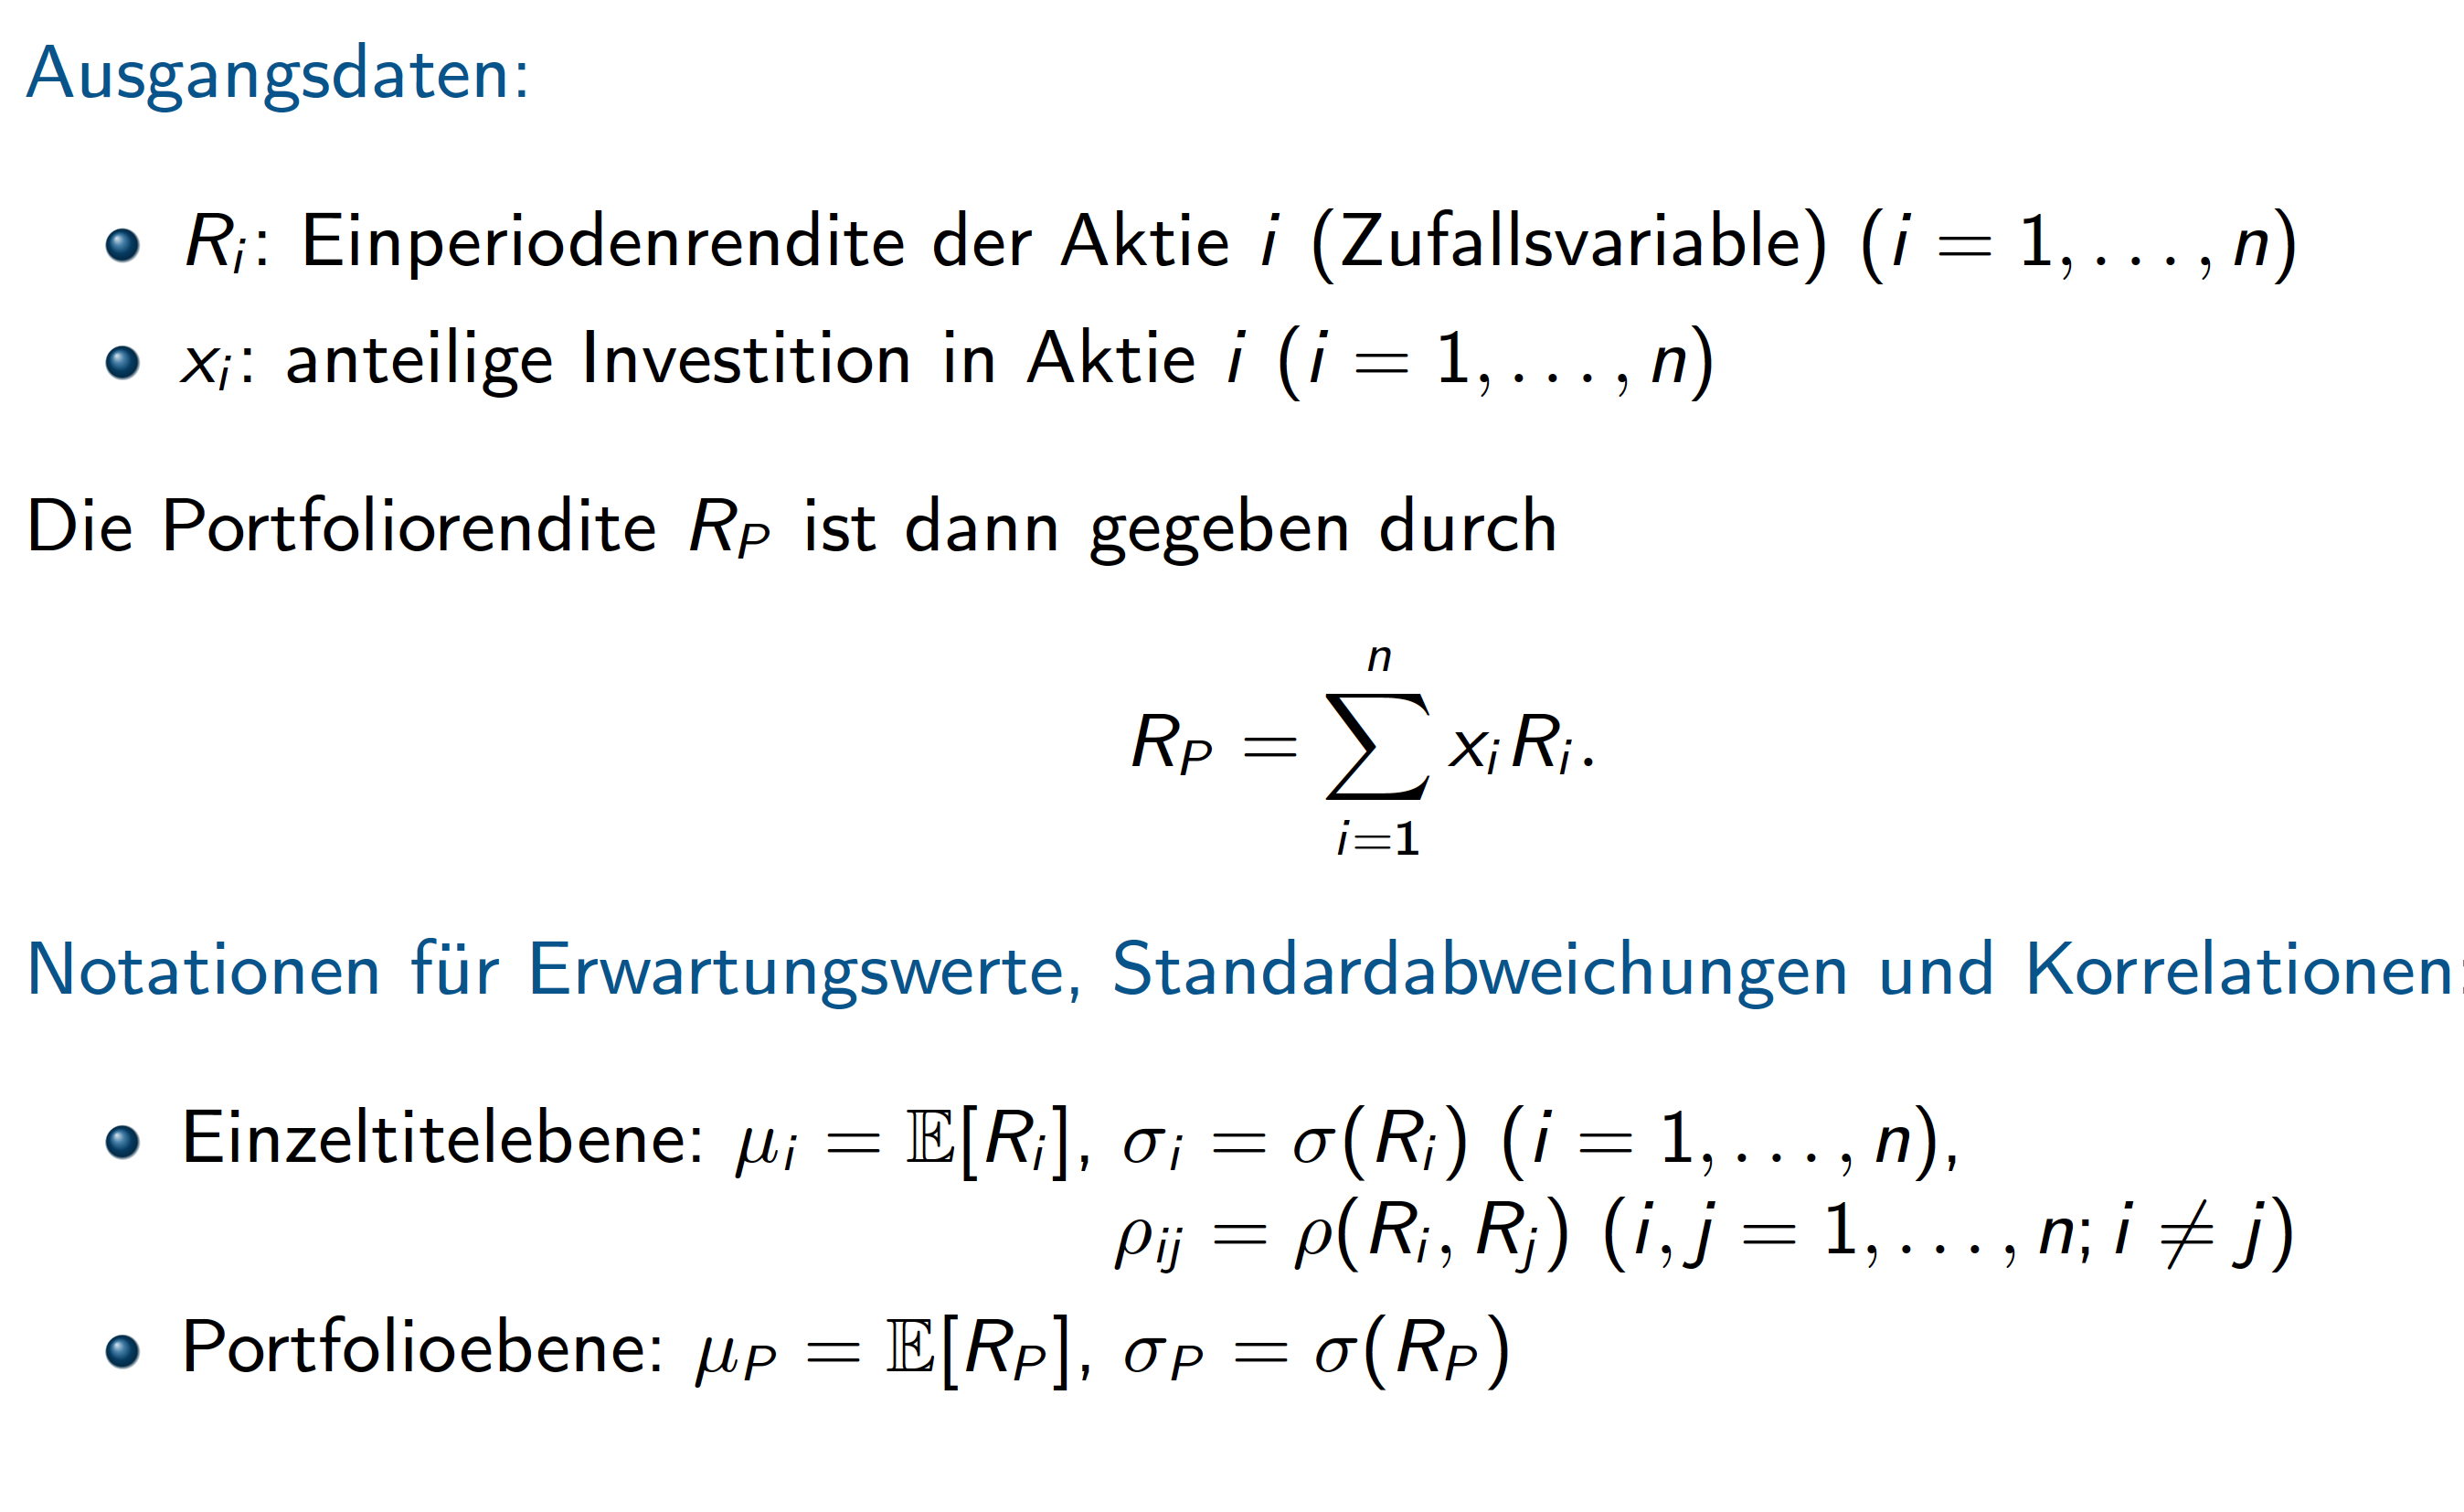
\includegraphics[width=\textwidth]{Bilder/Ausgangsdaten.png}
\end{figure}

\subsection{Effiziente Portfolios}

\begin{figure}[H]
\centering
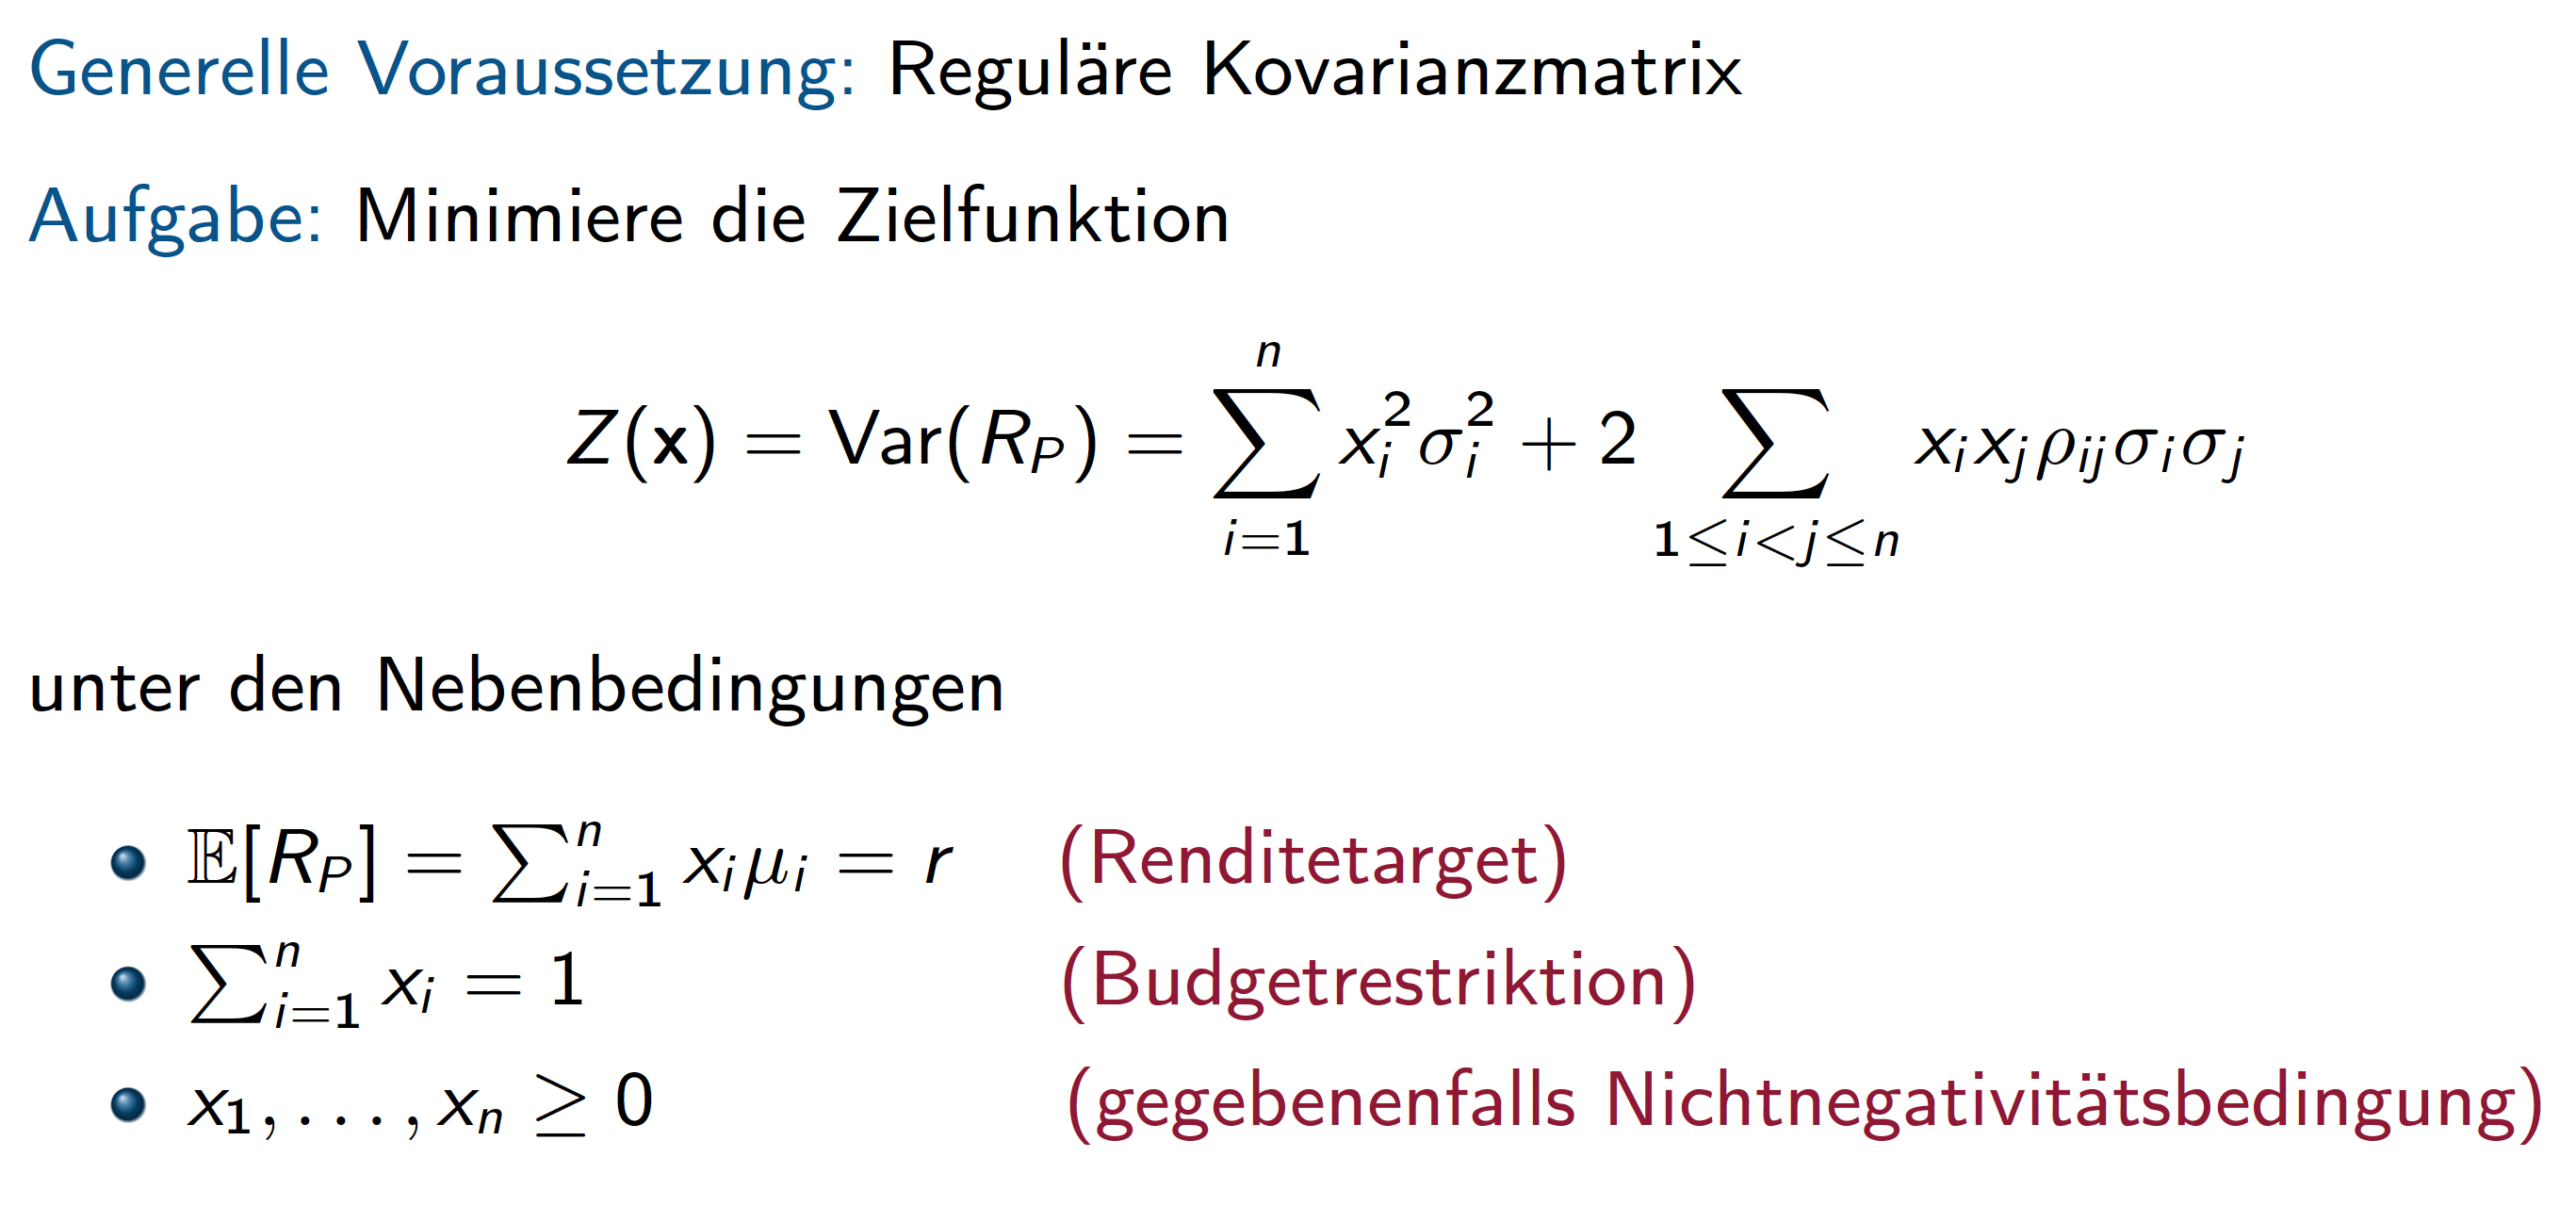
\includegraphics[width=\textwidth]{Bilder/Minimierungsproblem.png}
\end{figure}

\begin{itemize}
	\item Fall 1: Short Sales Allowed, L\"osung mit Lagrange-Ansatz, lokalen Extremwert der Lagrange-Funktion bestimmen
	\begin{itemize}
		\item geometrischer Rand der Menge aller zul\"assigen Portfolios besteht aus den Punkten, die bez\"uglich eines fixierten Erwartungswerts eine minimale Varianz aufweisen
		\item geometrischer Rand ist eine Wurzelfunktion (als Funktion von $\sigma^2$, bzw. der rechte Ast der Hyperbel (als Funktion von $\sigma^2$
		\item der effiziente Rand entspricht dem oberen Ast der Kurve inklusive dem global varianzminimalen Portfolio
	\end{itemize}
	\item Fall 2: No Short Sales, Quadratische Programmierung, i.A. keine analytische L\"osung, numerische Verfahren
\end{itemize}

\subsubsection{Alternative Formulierungen des Problems}

\begin{figure}[H]
\centering
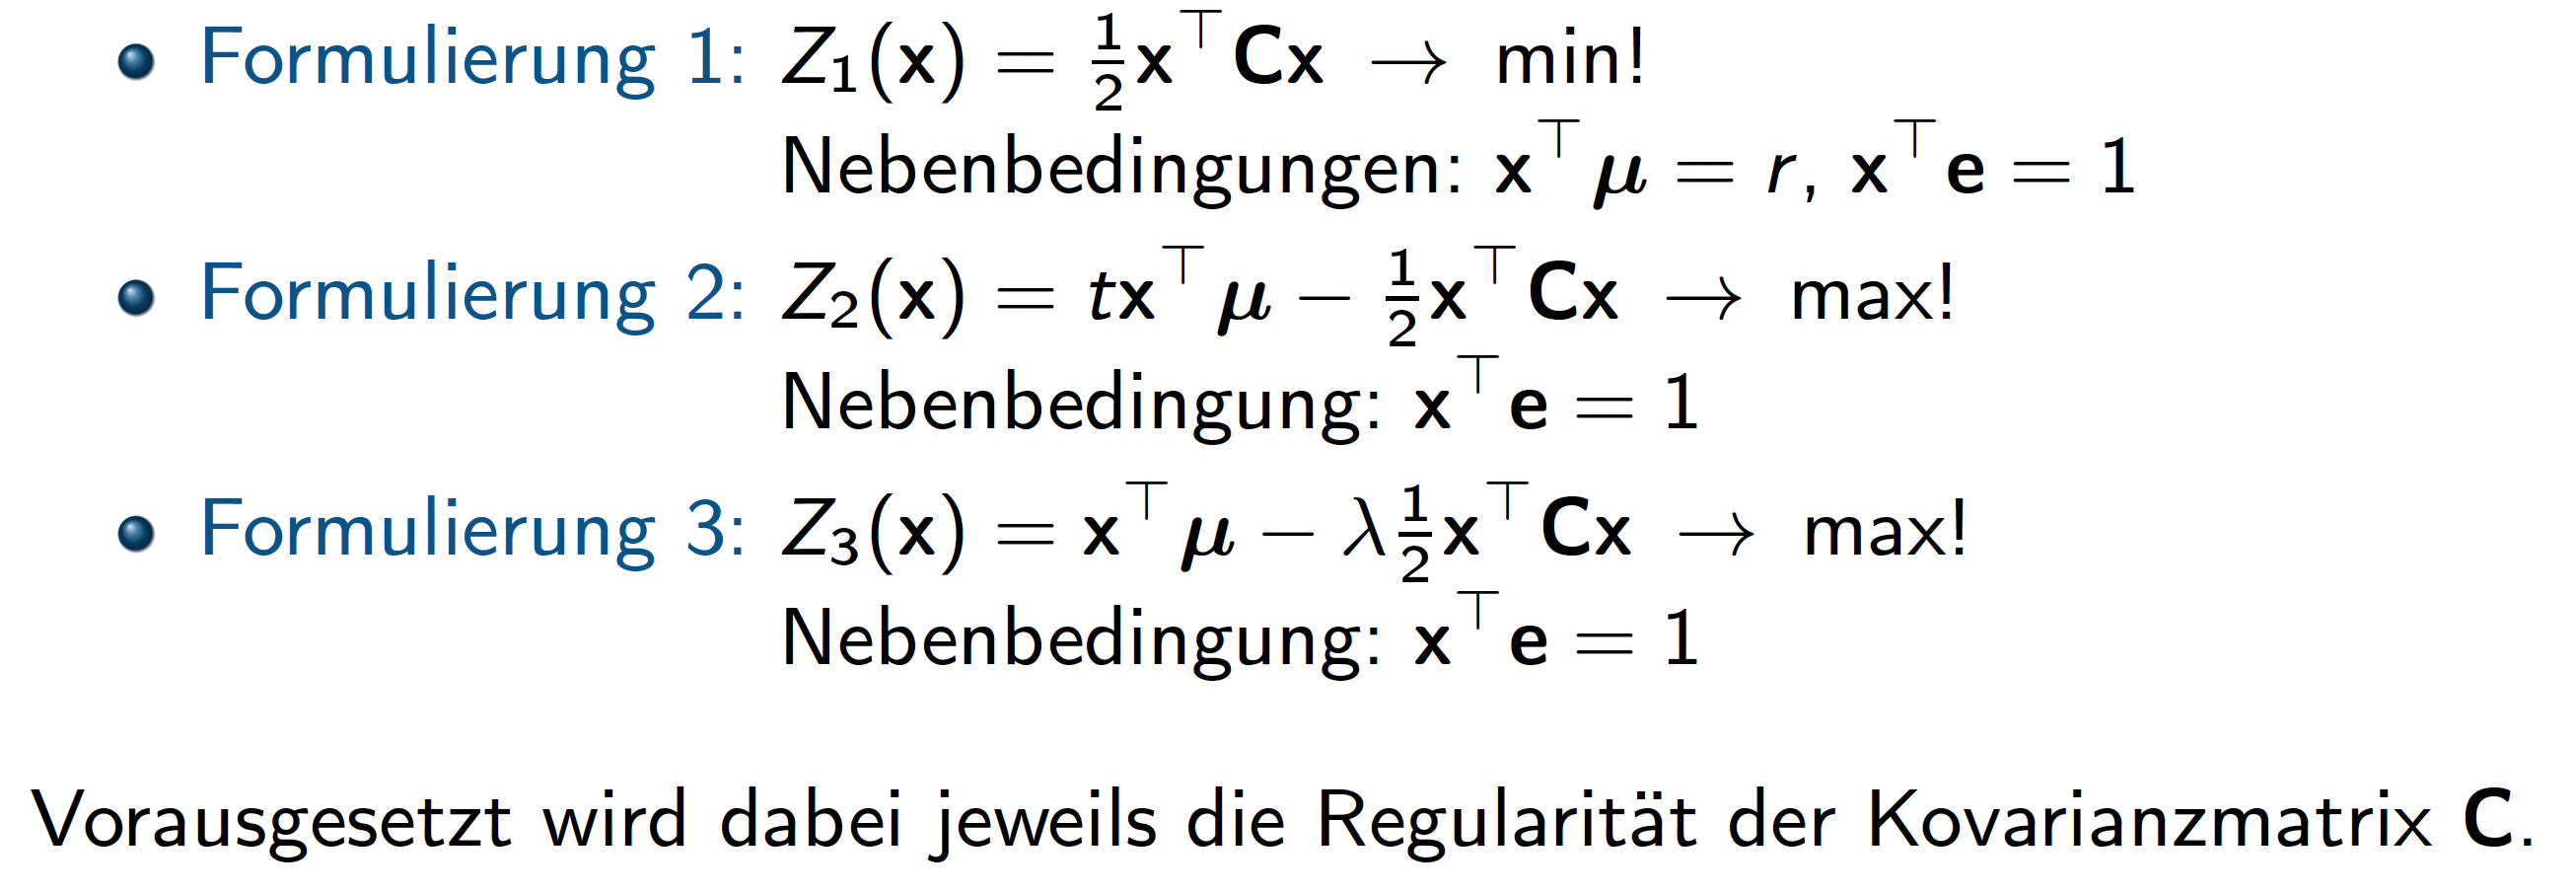
\includegraphics[width=\textwidth]{Bilder/alternativeFormulierungen.png}
\end{figure}

\begin{itemize}
	\item Lagrange-Funktion f\"ur Formulierung 2: \\ $L(x, \lambda) = tx^T \mu - \frac{1}{2} x^T Cx - \lambda (x^T e - 1)$ 
\end{itemize}

Fallstudie? \\

\subsection{Portfolioselektion}
























\end{document}
